\documentclass{article}

\usepackage[english]{babel}
\usepackage[utf8]{inputenc}
\usepackage{amsmath,amssymb}
\usepackage{parskip}
\usepackage{graphicx}
%\usepackage{subcaption}
\usepackage{amsmath}
\usepackage{float}
\usepackage{mathtools}

%\usepackage{subfig}
\usepackage[dvipsnames]{xcolor}
\usepackage[justification=centering]{caption}

\usepackage{subcaption}
\captionsetup{compatibility=false}
\usepackage{hyperref}


% Margins
\usepackage[top=2cm, left=2.5cm, right=2.5cm, bottom=3.0cm]{geometry}
% Colour table cells
%\usepackage[table]{xcolor}

%\colorlet{myBlue}{blue!10!black!10!}
%\colorlet{myBlue}{Violet}
\definecolor{myBlue}{HTML}{0000CC}

% Get larger line spacing in table
\newcommand{\tablespace}{\\[1.25mm]}
\newcommand\Tstrut{\rule{0pt}{2.6ex}}         % = `top' strut
\newcommand\tstrut{\rule{0pt}{2.0ex}}         % = `top' strut
\newcommand\Bstrut{\rule[-0.9ex]{0pt}{0pt}}   % = `bottom' strut


\def\one{\mbox{1\hspace{-4.25pt}\fontsize{12}{14.4}\selectfont\textrm{1}}}

%%%%%%%%%%%%%%%%%
%     Title     %
%%%%%%%%%%%%%%%%%
\title{HPC Project: Parallelizing a multilayer perceptron with openmp}
\author{Marian Aldescu - marian.aldescu@etu.univ-grenoble-alpes.fr}
\date{\today}

\begin{document}
	\maketitle
	
	\begin{abstract}
		Parallelizing the multilayer perceptron model has a great potential to improve the computation time, hence I show to what extent the program scales when increasing the number of threads, using openmp library in C++. After implementing the algorithm according to the original paper, the following step is to carefully identify the code regions  that can be executed in parallel. Finally, I show by measuring the time in different scenarios, that indeed, the training and testing of the neural network benefit from this. An interesting result is that the number of threads should be chosen depending on the network architecture.		
		
	\end{abstract}

Code: \url{https://github.com/marian-ald/hpc-mlp}
	
	\section{Design Methodology}
	
	
	\subsection{About the MLP}
	
	The work in this project is based on the first specification of a Multilayer Perceptron(MLP) given in \cite{rumelhart}, which is a method to learn patterns in a set of data, then generalize the rules on unseen samples, probably the most common notion in the field of deep learning.
	
	It is important to keep in mind that the name(\textit{multilayer perceptron}) may be misleading, since it does not use the perceptron algorithm for training, but the backpropagation algorithm. We detail the second later.
	
	
	Let's se what is the idea behind a MLP. For this, we refer to the notion of Artificial Neural Network(ANN), a method of learning inspired by the human brain. An ANN can be imagined as a directed graph, composed of layers, each of them containing a variable number of processing nodes(\textit{neurons}). Normally, nodes in the same layer are not connected between them, but only to nodes in the next layer. Edges are endowed with \textit{weights} and neurons with a \textit{threshold}(bias). First layer's number of nodes should match the size of input data, and the output layer's dimension is 1 or more, depending on the task. In Figure \ref{fig:mlp_1}, such an architecture can be seen.
	
	We need also to mention that the input of a neuron is computed as a linear combination of the neurons outputs from the previous layer, as in the 
	following equation:
	\begin{eqnarray}
		z_k = b_k + \sum_{i=1}^{n}w_{ki}x_i 
	\end{eqnarray}
	
	where $x_i \in \mathbb{R}^d$ is a training sample, $z_k$ is the neuron's value after the linear function is applied on it, $b_k$ is the neuron's bias and $w_{ki}$, the weights for all previous layer's neurons.
	
	The interesting part that makes ANNs so powerful is the non-linearity  applied on the neuron's linear function, and it is usually one of the: sigmoid, tanh, ReLU, softmax. They are usually chosen depending on the task at hand. If considering the sigmoid function, the activation($a_k$) looks as in Eq.(2).
	\begin{eqnarray}
		a_k = \sigma(z_k) = \frac{1}{1+e^{-z_k}} 
	\end{eqnarray}
	
	
	\begin{figure}[htbp]
		\centering
		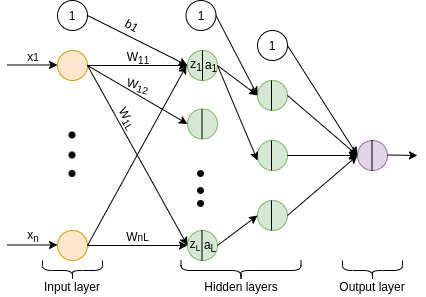
\includegraphics[scale=0.6]{fig/MLP.png}
		\caption{General architecture of a MLP with n inputs, 2 hidden layers and 1 output. One auxiliary node is added per layer to support the bias.}
		\label{fig:mlp_1}
	\end{figure}
	
	Another essential aspect and probably the most important one is the cost function, also know as the objective that we want to minimize over the entire data set. There are different cost functions, but as in the original paper\cite{rumelhart}, I used the \textit{sum of squared erros}, shown in Eq.(3), where $y_i$ is the expected label and $f(x_i)$ the predicted value for sample $x_i$. We multiply it with $\frac{1}{2}$, as it will facilitate the computation of the gradient later.
	\begin{eqnarray}
		E = \frac{1}{2} \sum_{i=1}^{N}(y_i - f(x_i))
	\end{eqnarray}
	
	
	Now that we have defined the structure of MLP, let's describe the behavior by which the learning happens. It can be split in 2 steps: \textit{forward propagation} and \textit{backward propagation}.\\
	
	
	
	\subsection{Forward propagation as a task parallelism model}
	It consists of feeding each sample of the data set to the NN, layer by layer, until the last one, when the error is calculated. We saw previously that in a MLP, nodes acts a processing units: they compute the linear function and then, the activation of a neuron, therefore we can see them as small tasks that can be run in parallel(Eq.4), with the mention that only operations of the same layer are able to run at the same time, as one layer depends on the previous layer's computation. Edges of the NN are "streams" of data, which at the same time apply their associated weights on the flow.
	
	\begin{equation}
		\text{	Run in parallel }
		\begin{cases}
			z_1 = b_1 + \sum_{i=1}^{n}w_{1i}x_i \\
			...\\
			z_K = b_K + \sum_{i=1}^{n}w_{Ki}x_i 
		\end{cases}       
		\iff z = W^\top \times x	
	\end{equation}
	
	where $z_1, ..., z_k$ are the values of the neurons in a layer of size $K$, and their computation can be formulated as a matrix multiplication, where $W$ contains the biases of neurons on the first row and $x$ contains value 1 on the first position, then the values of $\vec{x}$.
	
	For a layer, its activations(Eq.5) could also be computed in parallel, but I choose no to do this, as normally it doesn't have a large number of 
	neurons(usually, maximum the order of thousands), since the parallelization
	\begin{equation}
		a = 
		\begin{bmatrix}
			\sigma(z_1)  \\
			...  \\
			\sigma(z_k)
		\end{bmatrix}
	\end{equation} of this section, which introduces an overhead caused by the creation of the threads, may worsen the computation time. 
	
	
	\subsection{Backward propagation as a task parallelism model}
	
	Shortly, this step aims to adjust the weights of the MLP according to the training error, using a method called \textit{gradient descent algorithm}(GDA), that tries to find the global minima of the objective function, equivalent to a minimum probability to mistake.
	We need also to consider that, since we introduced non-linear operations in the model(sigmoid), it's very likely to have multiple local minima, preventing GDA to reach the lowest point.
	
	Performing the backpropagation phase helps us to answer the question: \textit{how much does the error change when the weights are changed by a small amount?} But the error $E$ does not depend directly on $w$, but on the activation $a$, and $a$ depends on $z$. This intuition leads to Eq.6, also know as \textit{chain rule}.
	\begin{eqnarray}
		\frac{\partial E}{\partial w^{(L)}} = \frac{\partial E}{\partial a^{(L)}} \times \frac{\partial a^{(L)}}{\partial z^{(L)}} \times \frac{\partial z^{(L)}}{\partial w^{(L)}}
	\end{eqnarray}
	where L is the last layer of the network. Knowing $E$ from Eq.3, we deduce easily that:
	\begin{eqnarray}
		\frac{\partial E}{\partial a^{(L)}} = a^{(L)} - y
	\end{eqnarray}
	Considering $a$ - the sigmoid function, its derivative w.r.t $z$ is:
	\begin{eqnarray}
		\frac{\partial a^{(L)}}{\partial z^{(L)}} = a^{(L)}(1 - a^{(L)})
	\end{eqnarray}
	The linear function $z$ can be seen as a polynomial of degree 1, hence:
	\begin{eqnarray}
		\frac{\partial z^{(L)}}{\partial w^{(L)}} = a^{(L-1)}
	\end{eqnarray}
	For all layers, starting from the last to the first, the partial derivative of $E$ w.r.t. the weights can be easily computed using chain rule, e.g. for the layer $L-1$, :
	\begin{eqnarray}
		\frac{\partial E}{\partial w^{(L-1)}} = \frac{\partial E}{\partial a^{(L)}} \times 
		\frac{\partial a^{(L)}}{\partial z^{(L)}} \times 
		\frac{\partial z^{(L)}}{\partial a^{(L-1)}} \times
		\frac{\partial a^{(L-1)}}{\partial z^{(L-1)}} \times 
		\frac{\partial z^{(L-1)}}{\partial w^{(L-1)}}
	\end{eqnarray}
	
	
	For any layer $L'$, we can compute the new weights using the well known \textit{gradient descent rule}:
	\begin{eqnarray}
		w^{(L')}_{ij} = 	w^{(L')}_{ij} - \eta \times \frac{\partial E}{w^{(L')}_{ij}}
	\end{eqnarray}
	where $\eta$ is the learning rate, which quantify how much the gradient vector will advance for each training sample.
	
	I split Eq. 11 in 3 steps: computing gradients, computing corrections, applying corrections, executed in this order, but inside each of the 3 tasks, the computation can be done in parallel, since the weights of the same layer are independent of each other. We can visualize this in Figure \ref{fig:back}.
	
	\begin{figure}[htbp]
		\centering
		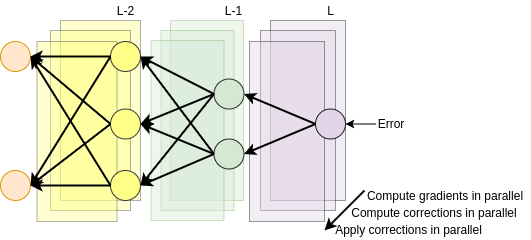
\includegraphics[scale=0.6]{fig/back_2.png}
		\caption{Backpropagation of the error. Each layer contains 3 parallel regions}
		\label{fig:back}
	\end{figure}
	
	\newpage
	
	Similar to the forward propagation, we can associate operations to nodes, like computing the partial derivatives, and then, edges can be seen as streams, but this time, they transport the gradients in the opposite direction, from the last layer to the first one. Therefore the backpropagation phase could be considered also a task parallelism model.
	
	Behind a NN, for both forward and backward propagation steps, there lie multiple regions with nested \textit{for} loops, so for this reason, the parallelization using \textit{openmp} is quite intuitive and easy.
	
	In my code there are several simple \textit{for} loops(non-nested) and I chose to keep them sequential, as they do not go over large array(like number of neurons in a layer), so their parallelization would not produce significant time improvement.
	
	Because the memory management is also important, in my implementation I chose to dynamically allocate the arrays used to store the network weights, gradients, etc., rather than using C++ \textit{vector} data structure, which could have a large memory footprint. At the end of the program, I free all the allocated memory.
	
	\section{Results/Data Analysis}
	
	I intended to test the neural network on a classification task, aiming to predict weather a patient is likely to suffer from heart disease or not. The data set\footnote{https://api.apispreadsheets.com/api/dataset/heart-disease/}, 
	containts 303 entries, each one having 13 attributes, which are different body measurements/indicators.
	All columns contain numerical values from distinct ranges, hence the min-max normalization was necessary to transfer them in [0,1] interval.
	For training, 80\% of the data was used, the rest being reserved for testing. In order to measure the performance, I used the accuracy measurement.
	
	
	I need to say from the beginning that after performing some tests, I came to the conclusion that my network doesn't succeed to learn. It seems that for the same hyperparameters, but for different trainings, it predicts all values as 0 and sometimes all testing samples are labeled as 1.
	Since the only difference was the initial values of the weights, I thought that maybe the problem could be the vanishing/exploding of the gradients, therefore I made sure that the weights initialization is done so that their histogram fits the normal distribution. Because the activation is the sigmoid function, I performed Xavier weights allocation, as in Eq.12. In Figure \ref{fig:normal} we can see an example of the weights allocation.
	\begin{eqnarray}
		w^{(L)} = random([size^{(L)}, size^{(L-1)}]) \times \sqrt{\frac{2}{size^(L)+size^{(L-1)}}}
	\end{eqnarray}
	
	Normally, k-fold cross validation needs to be employed, in order to find the optimal hyperparameters, but I reduced it to manually testing different values, due to lack of time and the need of elaboration when writing C++ code.
	
	The good part is that even if the trained model lacks accuracy, we can still measure the performance of parallelization.
	
	\begin{figure}[htbp]
		\centering
		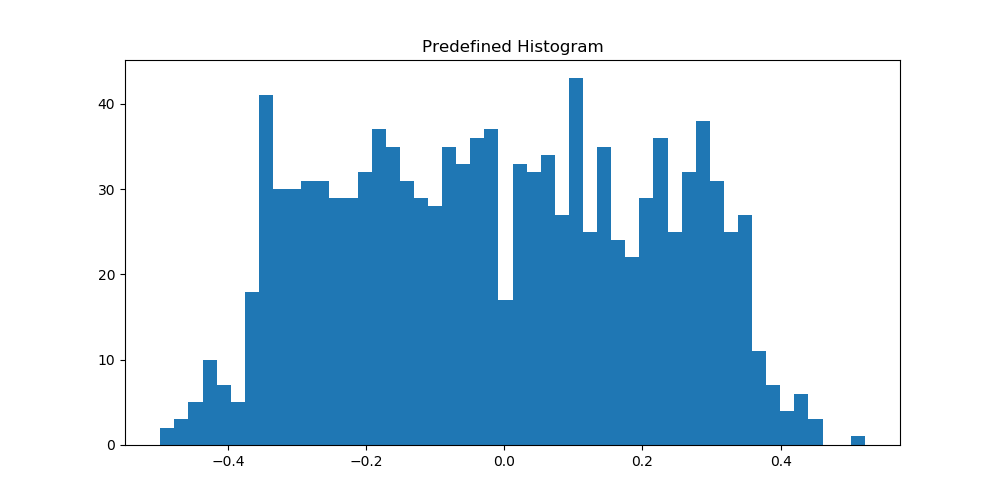
\includegraphics[scale=0.6]{fig/weights_1.png}
		\caption{Distribution of the initial weights values}
		\label{fig:normal}
	\end{figure}
	
	I run the tests on my personal computer, which has an i5 CPU with 2 cores, 2 threads/core, thus 4 threads and 1.7GHz frequency.
	
	When building the tests, I was interested to find out if the computation time scales for different number of cores and how does it scale for distinct neural network architectures.
	The results can be seen in Figure \ref{fig:results}. Looking at all 4 plots, we notice a good performance improvement by increasing the number of threads from 1 to 2.
	Also, we can see another interesting aspect, comparing the first 2 plots with the last 2. The architectures shown in Figure \ref{fig:results}(a) and \ref{fig:results}(b) focus on a NN with smaller, but more frequent layers. In both of them, we notice that when increasing the number of threads to 4, the performance doesn't change or is worse, due to the fact that each new layer in the NN means an additional fork/join, causing a time overhead. At the same time, the number of weights/layer is small, therefore, increasing the number of cores does not prove to be efficient.
	On the other hand, the second case (Figure \ref{fig:results}(c) and \ref{fig:results}(d)) focus on a NN with less layers but larger ones, hence, the threads spend more time computing rather than being created/deleted most of the time.
	
\begin{figure*}[t]
	\centering
	\hspace*{-9em}
	\begin{subfigure}[t]{.3\textwidth}
		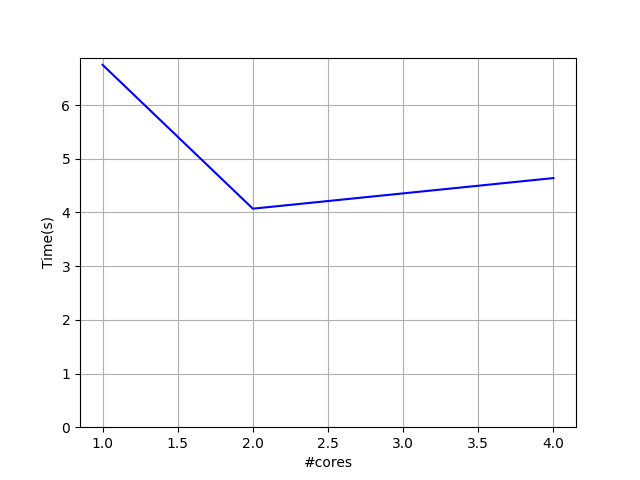
\includegraphics[scale=0.55]{fig/Figure_1.png}
			\parbox{8cm}{\caption{Hidden layers sizes: 50, 60, 50, 10}}
		\label{fig:c1}
	\end{subfigure}\hspace*{9.8em}
	\begin{subfigure}[t]{.3\textwidth}
		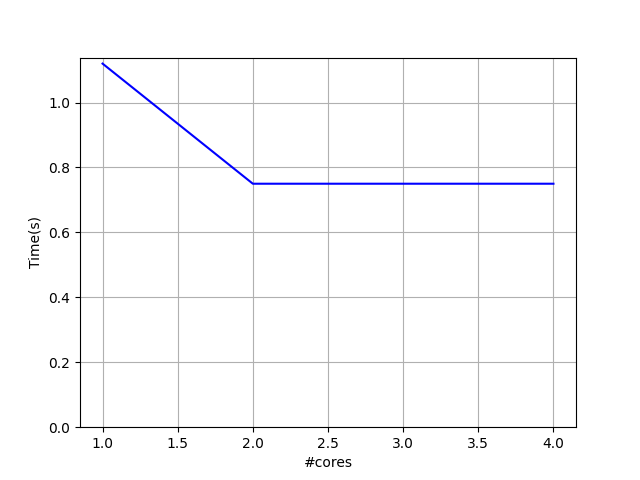
\includegraphics[scale=0.55]{fig/Figure_4.png}
		\parbox{8cm}{\caption[long]{Hidden layers sizes: 90, 70, 50, 20, 10}}	\label{fig:c2}
	\end{subfigure}
	
	\vspace*{-0.3em}
	
	\hspace*{-10em}
	\begin{subfigure}[b]{.3\textwidth}
		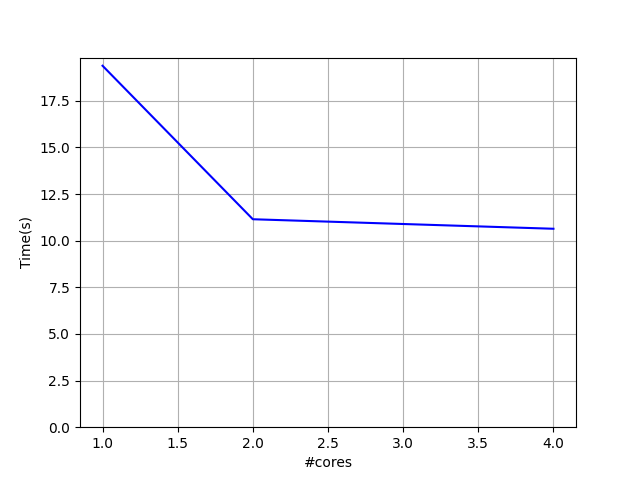
\includegraphics[scale=0.55]{fig/Figure_3.png}
		\parbox{8cm}{\caption{Hidden layers sizes: 200, 500}}
		\label{fig:c3}
	\end{subfigure}\hspace*{10.3em}
	\begin{subfigure}[b]{.3\textwidth}
		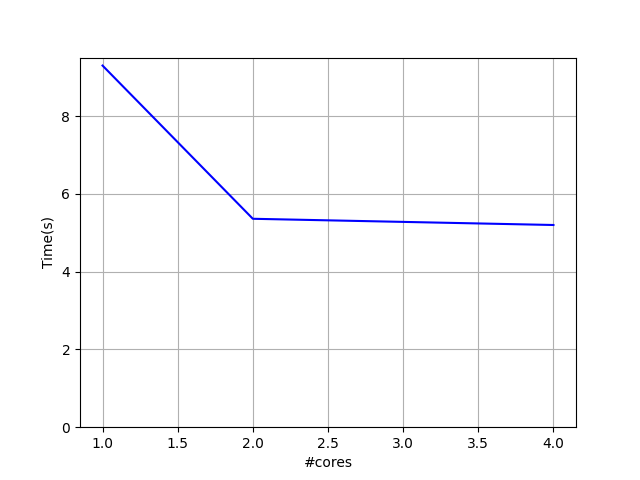
\includegraphics[scale=0.55]{fig/Figure_2.png}
		\parbox{8cm}{\caption[long]{Hidden layers sizes: 100, 2000}}
		\label{fig:c4}
	\end{subfigure}
	\caption{Time measurements of 4 different network architectures}
	\label{fig:results}
\end{figure*}
%	
\section{Conclusion}
In this project, I aimed to give an implementation of a multilayer perceptron, then to explore the possibility of improving its performance by parallelization. This consisted primarily in detecting the code regions that could be run in parallel, and at the same time to reason about the potential that by parallelizing them, the computation time would be reduced.

I mostly chose this project subject because I wanted to understand in detail how backpropagation algorithm works, not only in theory, but also in practice. I am happy for gaining a deeper knowledge about it, although it seems I still miss some aspects, since I could not succeed to make it actually learn something. On the other hand, the good part is that it still allowed me to prove that a time improvement can be achieved through parallelization, assuming that some eventual details that I missed do not affect the overall logic of the implementation.

The results that I have obtained show that my implementation of MLP scales when increasing the number of cores, and especially when the network has layers with high number of neurons, rather than more frequent and smaller layers.

To some extent, the project itself was a challenge for me, since implementing a NN in C++ is not easy, but in the end, I am satisfied that in the future I will use more confidently the existing implementations of deep learning algorithms from the well known libraries.


	\newpage
	
	\bibliographystyle{plain}
	\bibliography{bibliography}
	
	
	
\end{document}
